%!TEX root = ../../csuthesis_main.tex
\chapter{目标跟踪和意图识别算法验证}

\section{Carla 仿真平台与传感器配置}

Carla是Intel Labs和Computer Vision Center一同研发出来的一款开源自动驾驶仿真平台,它具有高保真度的城市地图,各类传感器模拟器,车辆物理引擎以及交通流管理机制,被广泛用于自动驾驶方面研究。因此本课题采用carla\_0.9.15版本仿真平台进行算法验证和仿真实验。

\subsection{仿真地图选择与场景设定}

本文选择 Carla 自带的两张典型城市地图:Town10HD 和 Town01 作为主要测试场景。

Town10HD 场景包含多车道城市道路、交通信号灯、交叉路口、障碍物遮挡、静态与动态交通参与者等复杂因素,适用于测试系统在高密度交通环境下的感知鲁棒性与行为分析准确性。

\begin{figure}[H]
	\centering
	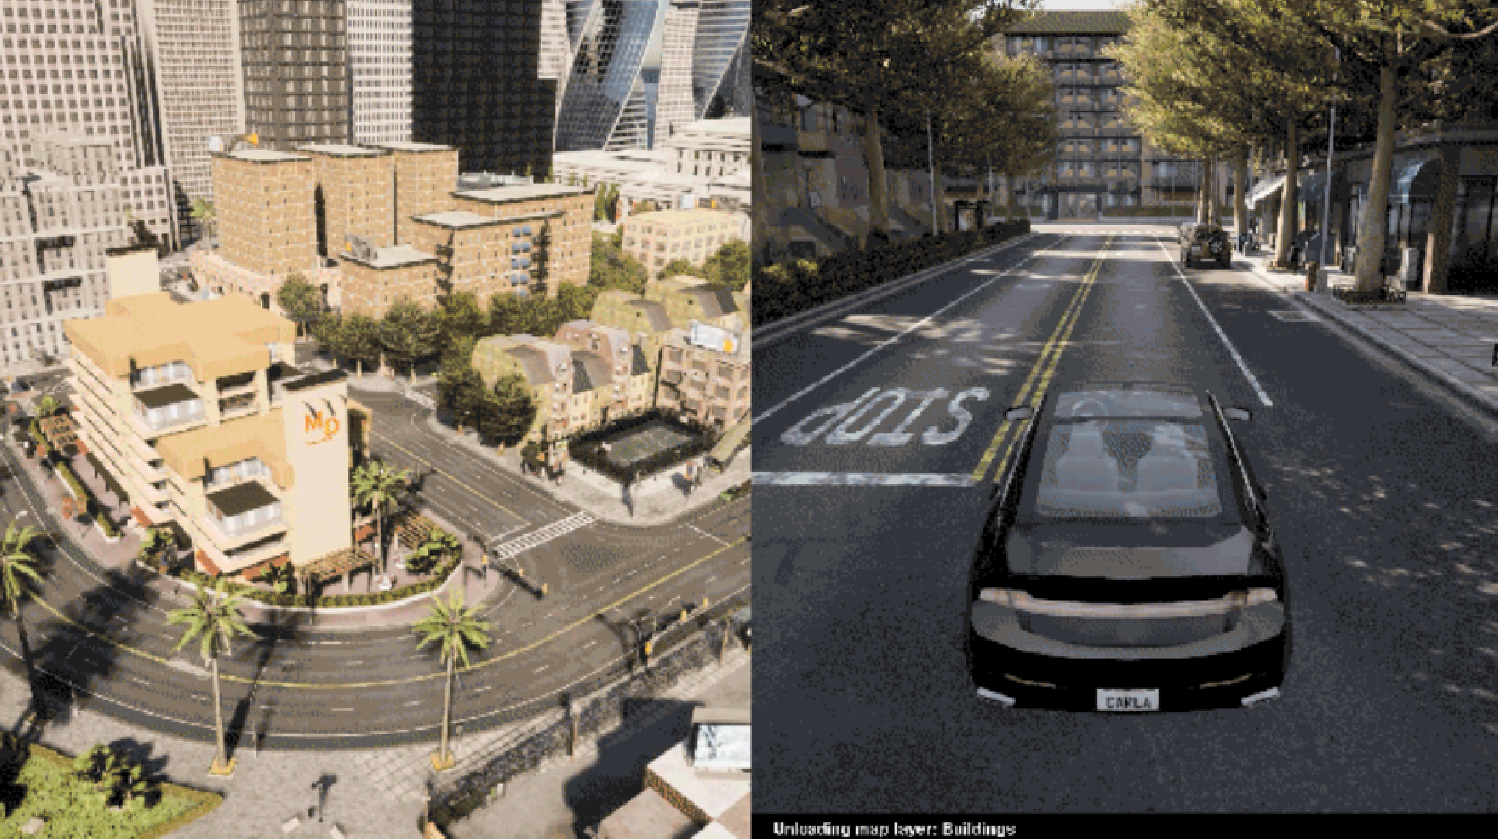
\includegraphics[width=0.8\textwidth]{images/图4 Town10HD地图展示.pdf}  % 引用转换后的 PDF 文件
	\caption{Town10HD地图展示}
	\label{fig:example_image}  % 可用于引用此图片
\end{figure}

Town01 场景则结构更为简单,适合用于算法功能验证与对比实验。

\begin{figure}[H]
	\centering
	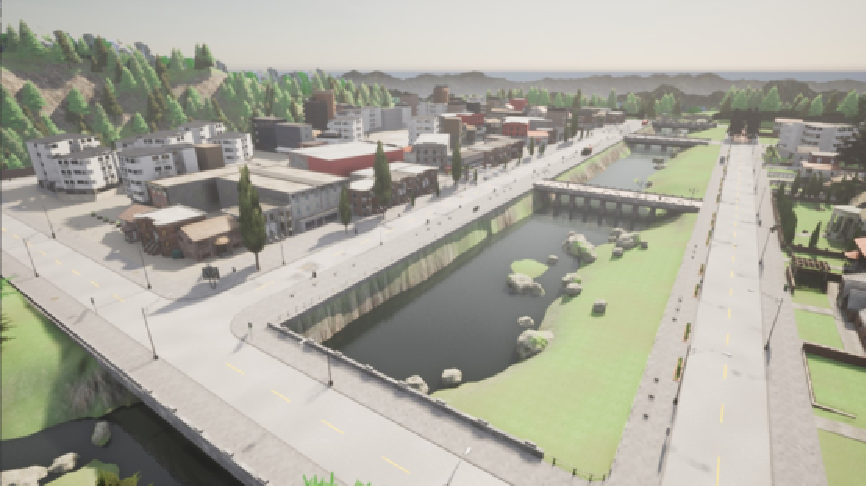
\includegraphics[width=0.8\textwidth]{images/图5 Town01地图展示.pdf}  % 引用转换后的 PDF 文件
	\caption{Town01地图展示}
	\label{fig:example_image}  % 可用于引用此图片
\end{figure}

仿真平台通过 Python API 方式加载地图并设置交通参与者生成密度与行为逻辑,确保每次启动后均可生成具有真实感的动态交通场景。

\subsection{本车模型与控制机制}

在系统初始化阶段,通过如下语句从 Carla 蓝图库中筛选车辆模型并生成本车:

\begin{figure}[H]
	\centering
	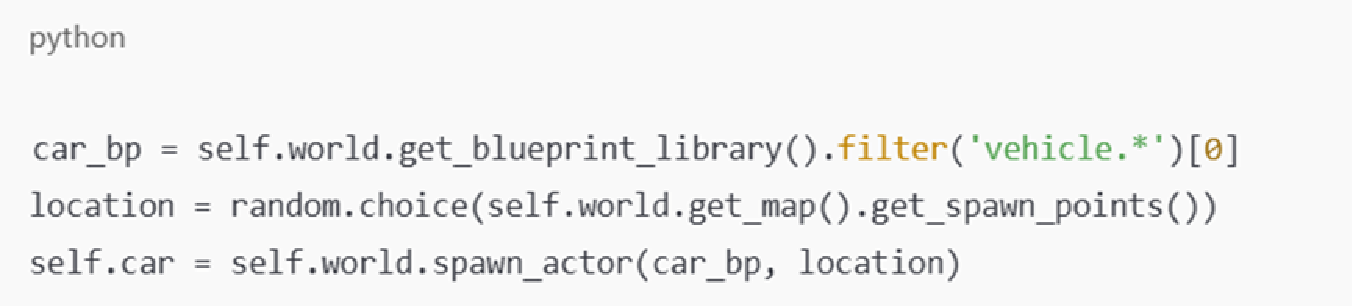
\includegraphics[width=0.8\textwidth]{images/图6 控制函数部分代码展示.pdf}  % 引用转换后的 PDF 文件
	\caption{控制函数部分代码展示}
	\label{fig:example_image}  % 可用于引用此图片
\end{figure}

车辆生成后系统对其施加控制命令,支持手动驾驶(通过键盘方向键操控)或接入后续自动控制模块。控制命令通过 Carla 的 car.apply\_control() 接口执行,包含油门、刹车、转向、手刹等基础控制量。

\subsection{摄像头传感器及其他配置说明}

为获取车辆前方图像信息,系统在本车前部安装一个 RGB 摄像头传感器,其参数配置如下:

\begin{table}[H]
	\caption{摄像头参数配置表}
	\label{tab:camera_params}
	\centering
	\begin{tabular}{ll}
		\toprule
		参数 & 数值 \\
		\midrule
		分辨率 & 960 × 540(与系统窗口相适配) \\
		视场角(FOV) & 90° \\
		安装位置 & 自车后方5.5米,高度2.8米 \\
		俯仰角 & -15°,向下略俯视 \\
		\bottomrule
	\end{tabular}
\end{table}

摄像头配置由camera\_bp.set\_attribute()函数完成,采集的图像数据通过监听函数 self.camera.listen() 注册至主控循环,每帧图像均可进行目标检测、跟踪与意图分析,并实时渲染至用户界面或保存为数据集。

要想让系统各个模块针对相同时间点的图像帧实施同步处理,本系统便开启Carla的同步仿真模式(synchronous\_mode=True),使得每一阶段环境状态的更新都能同传感器输出相对应,进而加强处理过程的可掌控性以及图像帧的稳定性,处于同步模式的时候,系统会按照固定频率(20FPS)去调用world.tick()以推动环境向前发展,这样就能保障传感器输出和控制行为之间存在确切的一一对应关系,有益于维持状态追踪的准确性并延续分析逻辑的连贯性。

而且,系统依靠pygame图形界面来做图像渲染工作,用numpy,cv2,json这些工具库执行图像处理,数据标注以及数据集形成方面的任务,整个系统要靠CarlaServer正常运行(直接在Windows下双击CarlaUE4.exe就能启动),从而保证模拟世界稳定又开放。

\subsection{环境与工具链}

为高效实现自动驾驶场景下的视觉目标跟踪与意图识别算法,并完成系统级仿真测试与可视化功能开发,本文构建了一个基于 Carla 仿真平台的完整算法开发与测试环境。本节将对本项目使用的软硬件配置、开发语言、核心依赖库与工具链进行说明。

\textbf{硬件平台:}实验采用配置如下表的工作站,满足实时仿真需求。

\begin{table}[H]
	\caption{硬件配置表}
	\label{tab:hardware_config}
	\centering
	\begin{tabular}{ll}
		\toprule
		组件 & 规格 \\
		\midrule
		CPU & Intel Core i7-10750H @ 2.60GHz \\
		GPU & NVIDIA RTX 2060 (6GB GDDR6) \\
		内存 & 16GB DDR4 \\
		存储 & 512GB NVMe SSD \\
		\bottomrule
	\end{tabular}
\end{table}

\textbf{软件与工具:}项目开发主要在 Windows 10 平台下进行。核心依赖环境和工具包括:

\begin{table}[H]
	\caption{软件工具链配置}
	\label{tab:software_stack}
	\centering
	\begin{tabular}{lll}
		\toprule
		软件 & 版本 & 用途 \\
		\midrule
		Python & 3.7.9 & 主控程序开发 \\
		Carla & 0.9.15 & 自动驾驶仿真 \\
		Pygame & 2.5.2 & 可视化界面渲染与用户交互界面 \\
		OpenCV & 4.8.0 & 图像读取与保存,数据集采集处理 \\
		deep\_sort\_realtime & 1.3.2 & 多目标跟踪(基于SIFT改进版) \\
		\bottomrule
	\end{tabular}
\end{table}

其中CarlaSimulator的安装与启动采用图形化模式,即双击启动CarlaUE4.exe来打开仿真服务端,而客户端代码运行时则是以TCP方式通信(默认端口2000),为保证数据同步性,系统均统一采用Carla的同步模式运行,使得传感器输出,车辆控制以及仿真时间能够严格对齐。

Python环境用Anaconda来做管理,创建单独的虚拟环境之后再通过pip install去装那些依赖库,这样就能保证版本稳定而且可重现,如OpenCV之类的库是从PyPI上获取的,或者按照官方GitHub上的源码执行安装。

\section{目标跟踪数据集与评价标准}

\subsection{数据集介绍}

本研究借助CARLA自动驾驶仿真平台来生成实验所需的目标跟踪数据集,从中挑选出其内置的Town01以及Town10这两个典型城市场景,以此模拟复杂交通环境下多目标的移动过程,借助仿真环境的自动标签功能,再结合同步采集的图像帧以及位置信息,构建起一个用于单目标及多目标跟踪任务的场景级数据集。该数据集总共包含6568张图像,涉及白天光照条件下不同车速、不同交通密度以及交叉路口场景。

数据集中的每一帧图像都含有时间戳、目标类别、目标唯一编号(ID)、二维边界框位置信息以及部分三维空间坐标信息,方便在后续实验里对目标进行轨迹拟合与跨帧关联,凭借对仿真场景的控制,保证了数据中目标在多个帧之间有连续运动特征,适合用于验证跟踪算法在遮挡、加速、转弯等动态情形下的稳定性与准确性。

为保证实验的通用性与可重复性,在数据采集过程中严格把控场景中的变量设置,比如交通流量密度、行人及非机动车的比例等,尽可能去还原真实城市道路环境,实验所用数据依据时间顺序被划分成训练集和测试集,在后续模型训练与评估中分别用于模型参数优化以及算法性能验证。

借助上述自建数据集的构建与清洗,为后续章节中目标跟踪算法的实验验证奠定了可靠基础,同时也为开展多场景、多气象条件下的扩展研究提供了实验支持。

\subsection{采集流程设计}

系统每一次执行仿真时,会自动搜集由模拟车载摄像头捕捉到的图像帧,并且立即从当前帧当中识别出其它行驶中的车辆目标,利用Carla给出的车辆状态接口,可以得到这些目标的三维坐标位置以及速度大小等数据,再通过转换矩阵把它们映射到摄像头图像所在的平面坐标系里面,从而生成适用于目标检测任务的二维边框形状。

为增强数据的多样性和实用性,系统设计了如下采集流程:

\textbf{(1)	图像获取:}定期(如每隔 5 帧)从主摄像头传感器中截取 RGB 图像;

\textbf{(2)	目标提取:}从当前帧中提取所有可见车辆,获取其三维边界框与速度;

\textbf{(3)	投影计算:}将三维框转换为图像平面坐标,形成二维检测框;

\textbf{(4)	追踪标记:}判断是否为当前正在追踪的目标,赋予唯一 ID;

\textbf{(5)	结果保存:}将图像帧以 JPG 格式保存,同时输出 JSON 格式的结构化标签文件。

此流程保证所采集的数据具备较高的时效性且带有完整的标签结构,从而能够应对后续诸如目标检测,跟踪以及行为识别之类的诸多任务需求。

\begin{figure}[H]
	\centering
	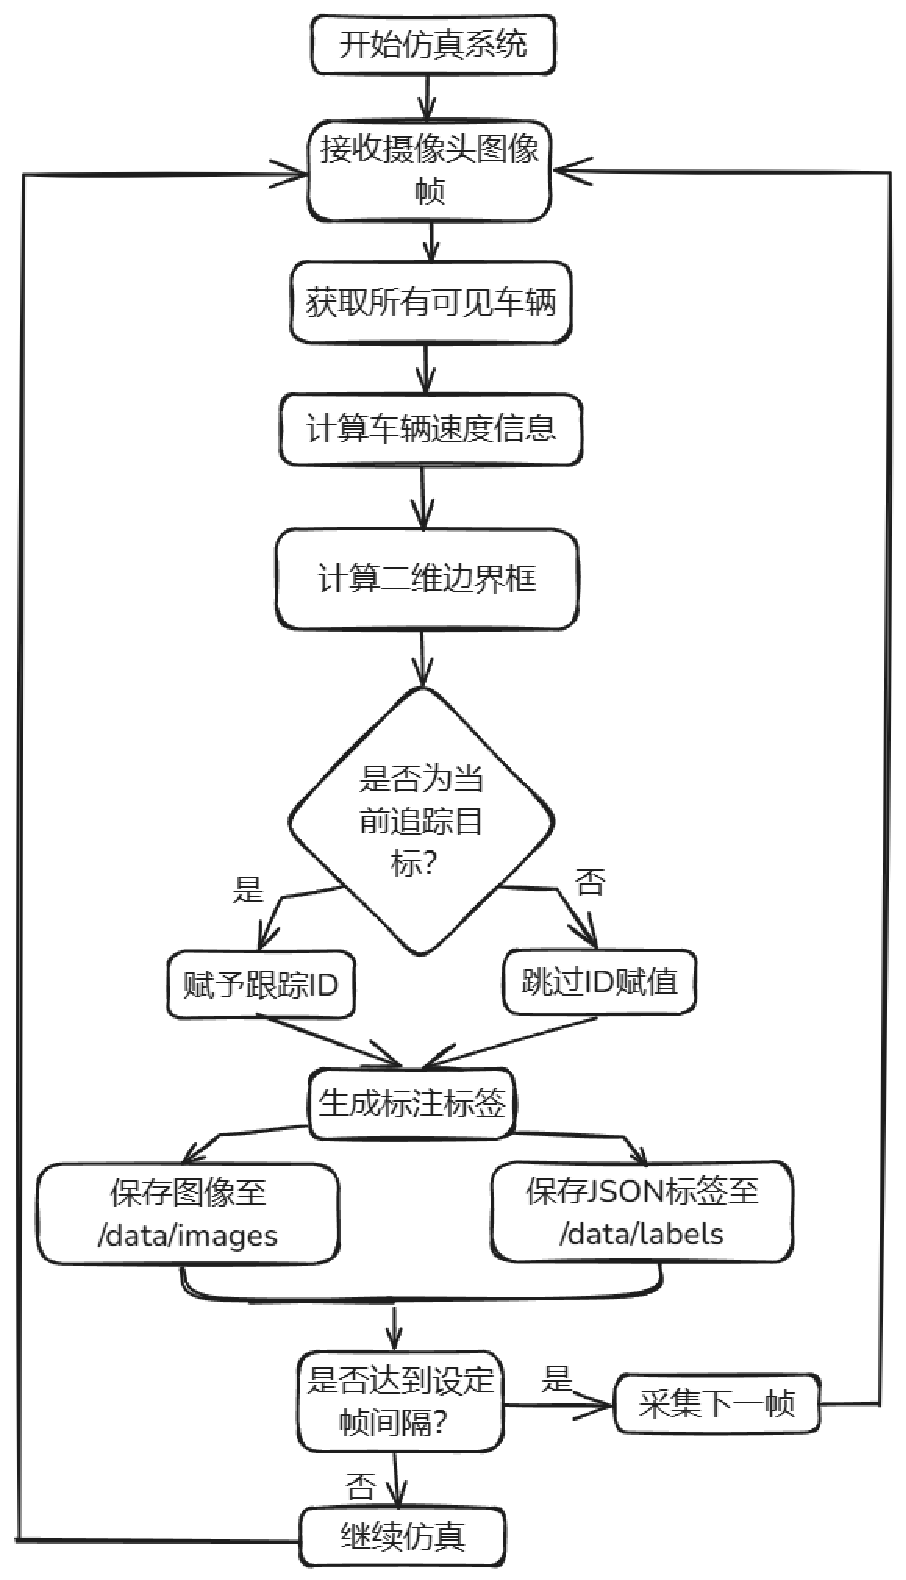
\includegraphics[height=0.55\textheight]{images/图7 数据采集流程图.pdf}  % 引用转换后的 PDF 文件
	\caption{数据采集流程图}
	\label{fig:example_image}  % 可用于引用此图片
\end{figure}

\subsection{标注信息结构设计}

每个 JSON 标签文件对应一帧图像,包含该图像中所有检测到的车辆目标。标签信息以列表形式记录,每一项包含如下字段:

\textbf{bbox:}二维边界框左上角起 4 个顶点的图像坐标;

\textbf{speed\_m\_s:}目标瞬时速度(单位为米每秒);

\textbf{tracked\_id:}若目标被当前追踪模型识别并持续跟踪,则记录其分配 ID,否则为 null。

此结构可容纳常用目标检测框架(诸如YOLO,FasterR - CNN)以及跟踪框架(诸如DeepSORT,ByteTrack)所必要的数据格式,而且能够被拓展应用到行为分析任务里的时序建模当中。

\begin{figure}[H]
	\centering
	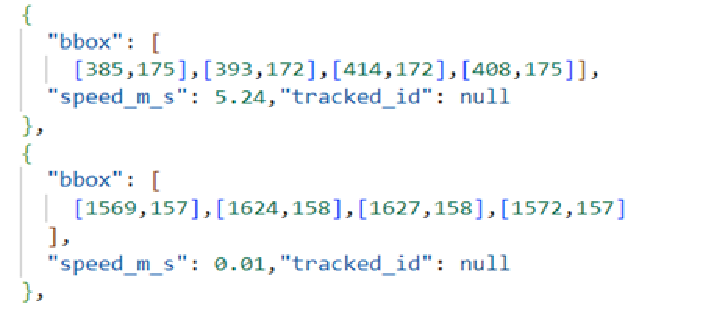
\includegraphics[width=0.8\textwidth]{images/图8 数据文件结构截图.pdf}  % 引用转换后的 PDF 文件
	\caption{数据文件结构截图}
	\label{fig:example_image}  % 可用于引用此图片
\end{figure}

\subsection{评价指标}

在官方MOT数据上进行目标跟踪算法的性能评估测试时,MOTA\cite{bernardin2008evaluating}和IDF1\cite{ristani2016performance}通常被认为是最重要的评估指标。和MOTA相关的指标囊括假阴性、假阳性以及ID切换率,这里面假阴性和假阳性属于检测结果,唯有ID切换跟跟踪存在关联,MOTA对检测器的性能更为关注,和MOTA不一样,IDF1更看重相关性以及一致性,并且主要借助轨道上正确的ID来计算F1值,当把跟踪算法与相同或者更小的ID切换做比较时,IDF1指示符更具代表性。以下是评估指标:

(1)IDF1:检测和跟踪对象中具有正确ID的检测对象的比例。
\begin{equation}
	IDF1 = \frac{2IDTP}{2IDTP + IDFP + IDFN},
\end{equation}

IDTP 可以看成是检测整个视频流中正确分配的目标的数量,IDFN可以检测到整个视频流中未分配的目标数量,IDFP则可以检测出整个视频中错误分配的目标数量。IDF1的值越大越好。

(2)IDP:识别准确率。
\begin{equation}
	IDP = \frac{IDTP}{IDTP + IDFP},
\end{equation}
识别准确率的值越大越好。

(3)IDR:识别召回率。
\begin{equation}
	IDR = \frac{IDTP}{IDTP + IDFN},
\end{equation}
识别召回率的值越大越好。 

(4)ID Sw:身份切换总数量。跟踪过程中身份切换的次数越少越好。 

(5)MOTA:该指标结合了三个误差项:误报,错过的目标和身份切换。
\begin{equation}
	MOTA = 1 - \frac{\sum_{t}(FN_{t} + FP_{t} + IDSW_{t})}{\sum_{t}GT_{t}},
\end{equation}

MOTA 的值主要由检测器的效果来决定,值越大代表检测器的效果更好,MOTA的值越大越好。 




\section{车辆跟踪效果分析}

\subsection{车辆跟踪精度分析}

在此次实验里,针对传统DeepSORT算法以及本文所改进的DeepSORT算法开展了对比测试,测试的场景涉及了无遮挡和有遮挡这两种典型情形,且都是基于CARLA仿真平台里的Town01城市场景与Town10城市场景进行的,经过精心安排的交通流模拟以及场景控制,保证了实验在复杂交通状况下有代表性以及可重复性。

在无遮挡的情形时,两种算法都可比较准确地对车辆目标实施检测与跟踪,如图呈现的那样,图的上半部分呈现的是DeepSORT算法的跟踪成果,下半部分则是本文改进算法的输出,两种方法在车辆正常行驶进程中都可为不同目标赋予稳定的ID标识,达成连续帧之间的目标关联。
\begin{figure}[H]
	\centering
	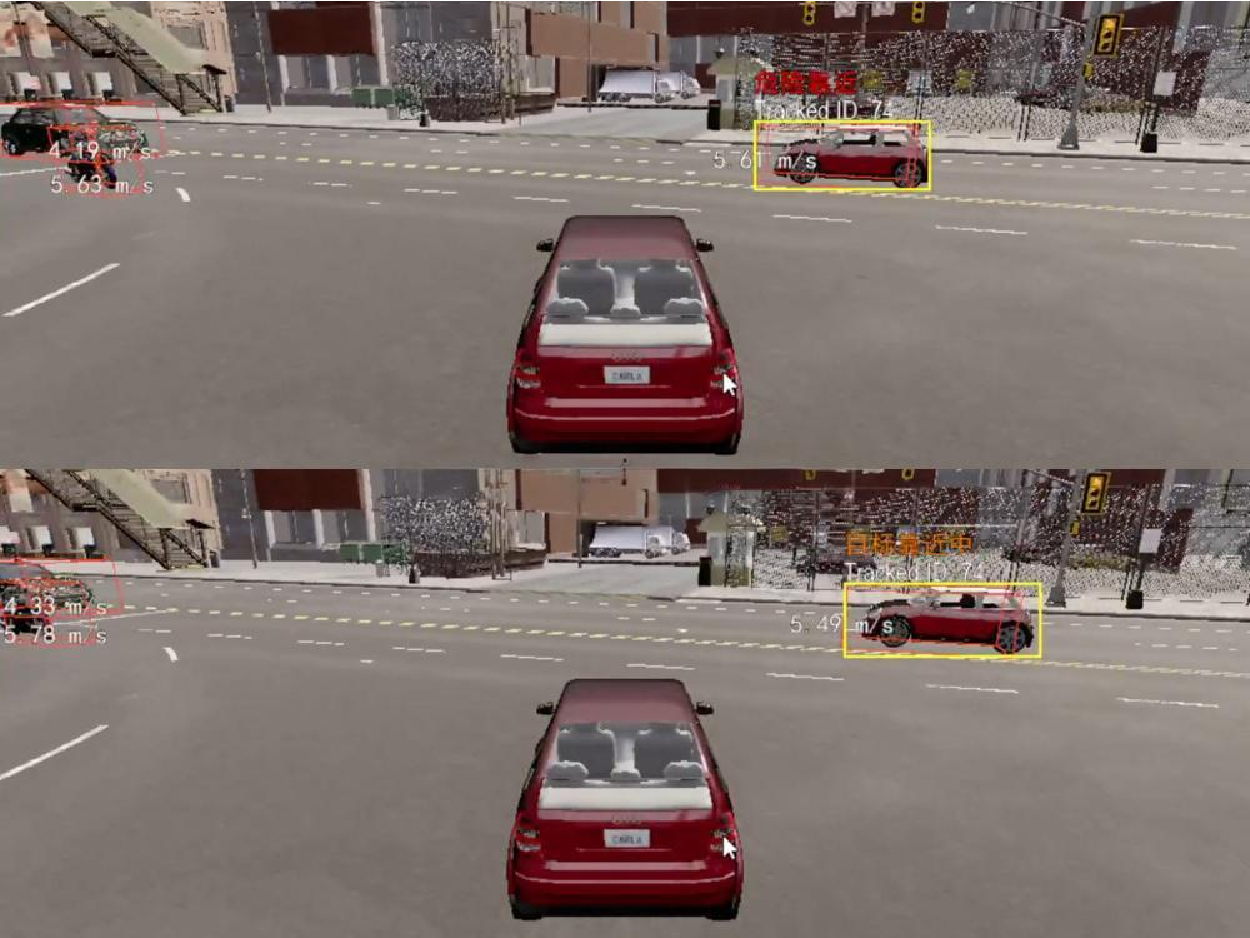
\includegraphics[width=0.8\textwidth]{images/未遮挡.pdf}  % 引用转换后的 PDF 文件
	\caption{无遮挡下跟踪效果对比}
	\label{fig:nocover}  % 可用于引用此图片
\end{figure}

下图~\ref{fig:covered1} 展示了在存在遮挡情况下的目标跟踪表现。在该实验场景中,车辆 ID=12被一颗树木在路口处部分遮挡,随后重新出现在摄像头视野中。DeepSORT 算法在遮挡发生后,短暂丢失了原始车辆的 ID,重新赋予了另外的编号,误将其识别为新目标。虽然在后续目标未被严重遮挡的帧中 DeepSORT 能够再次关联该目标,但在 ID 连续性方面存在明显断裂。
\begin{figure}[H]
	\centering
	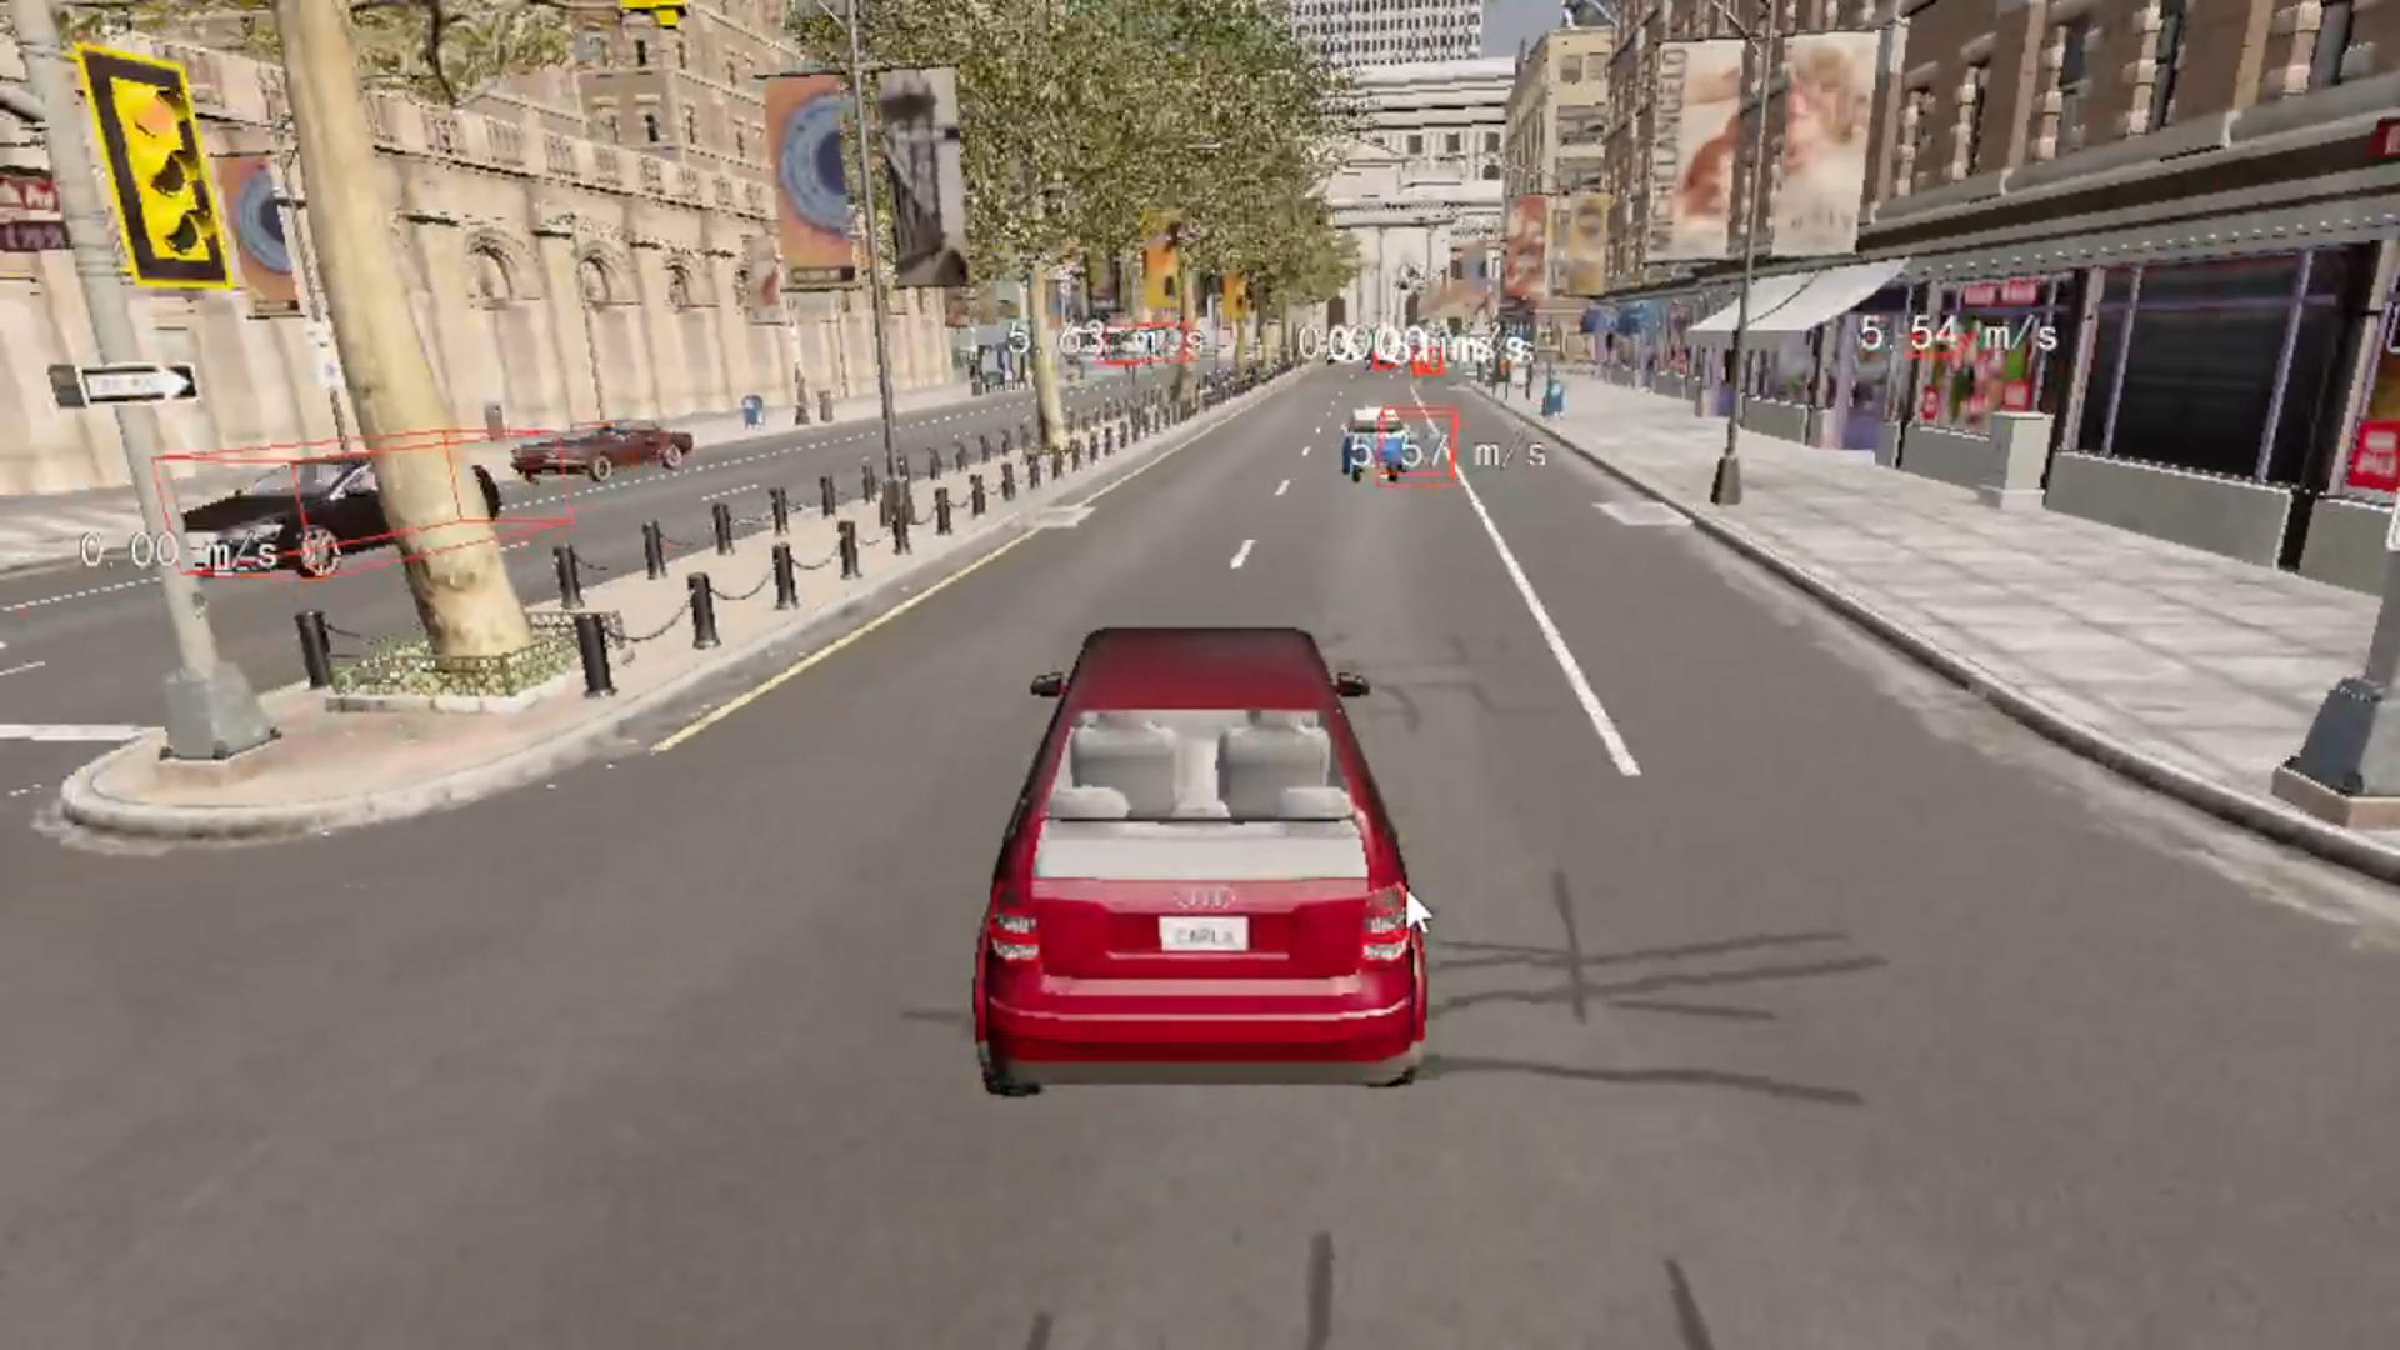
\includegraphics[width=1.0\textwidth]{images/遮挡未跟踪.pdf}  % 引用转换后的 PDF 文件
	\caption{遮挡下DeepSORT跟踪效果}
	\label{fig:covered1}  % 可用于引用此图片
\end{figure}

相较而言,本文所改进的算法在处理该遮挡事件之时呈现出更为强大的鲁棒性,当车辆ID=12出现部分遮挡情况后,目标不会丢失,算法依然可精准地识别并且跟踪其作为同一目标,同时保持原本的ID编号不发生改变,这意味着改进算法在特征匹配以及时间帧间关联机制方面得到了提高,提升了在复杂交通环境下的遮挡恢复能力。
\begin{figure}[H]
	\centering
	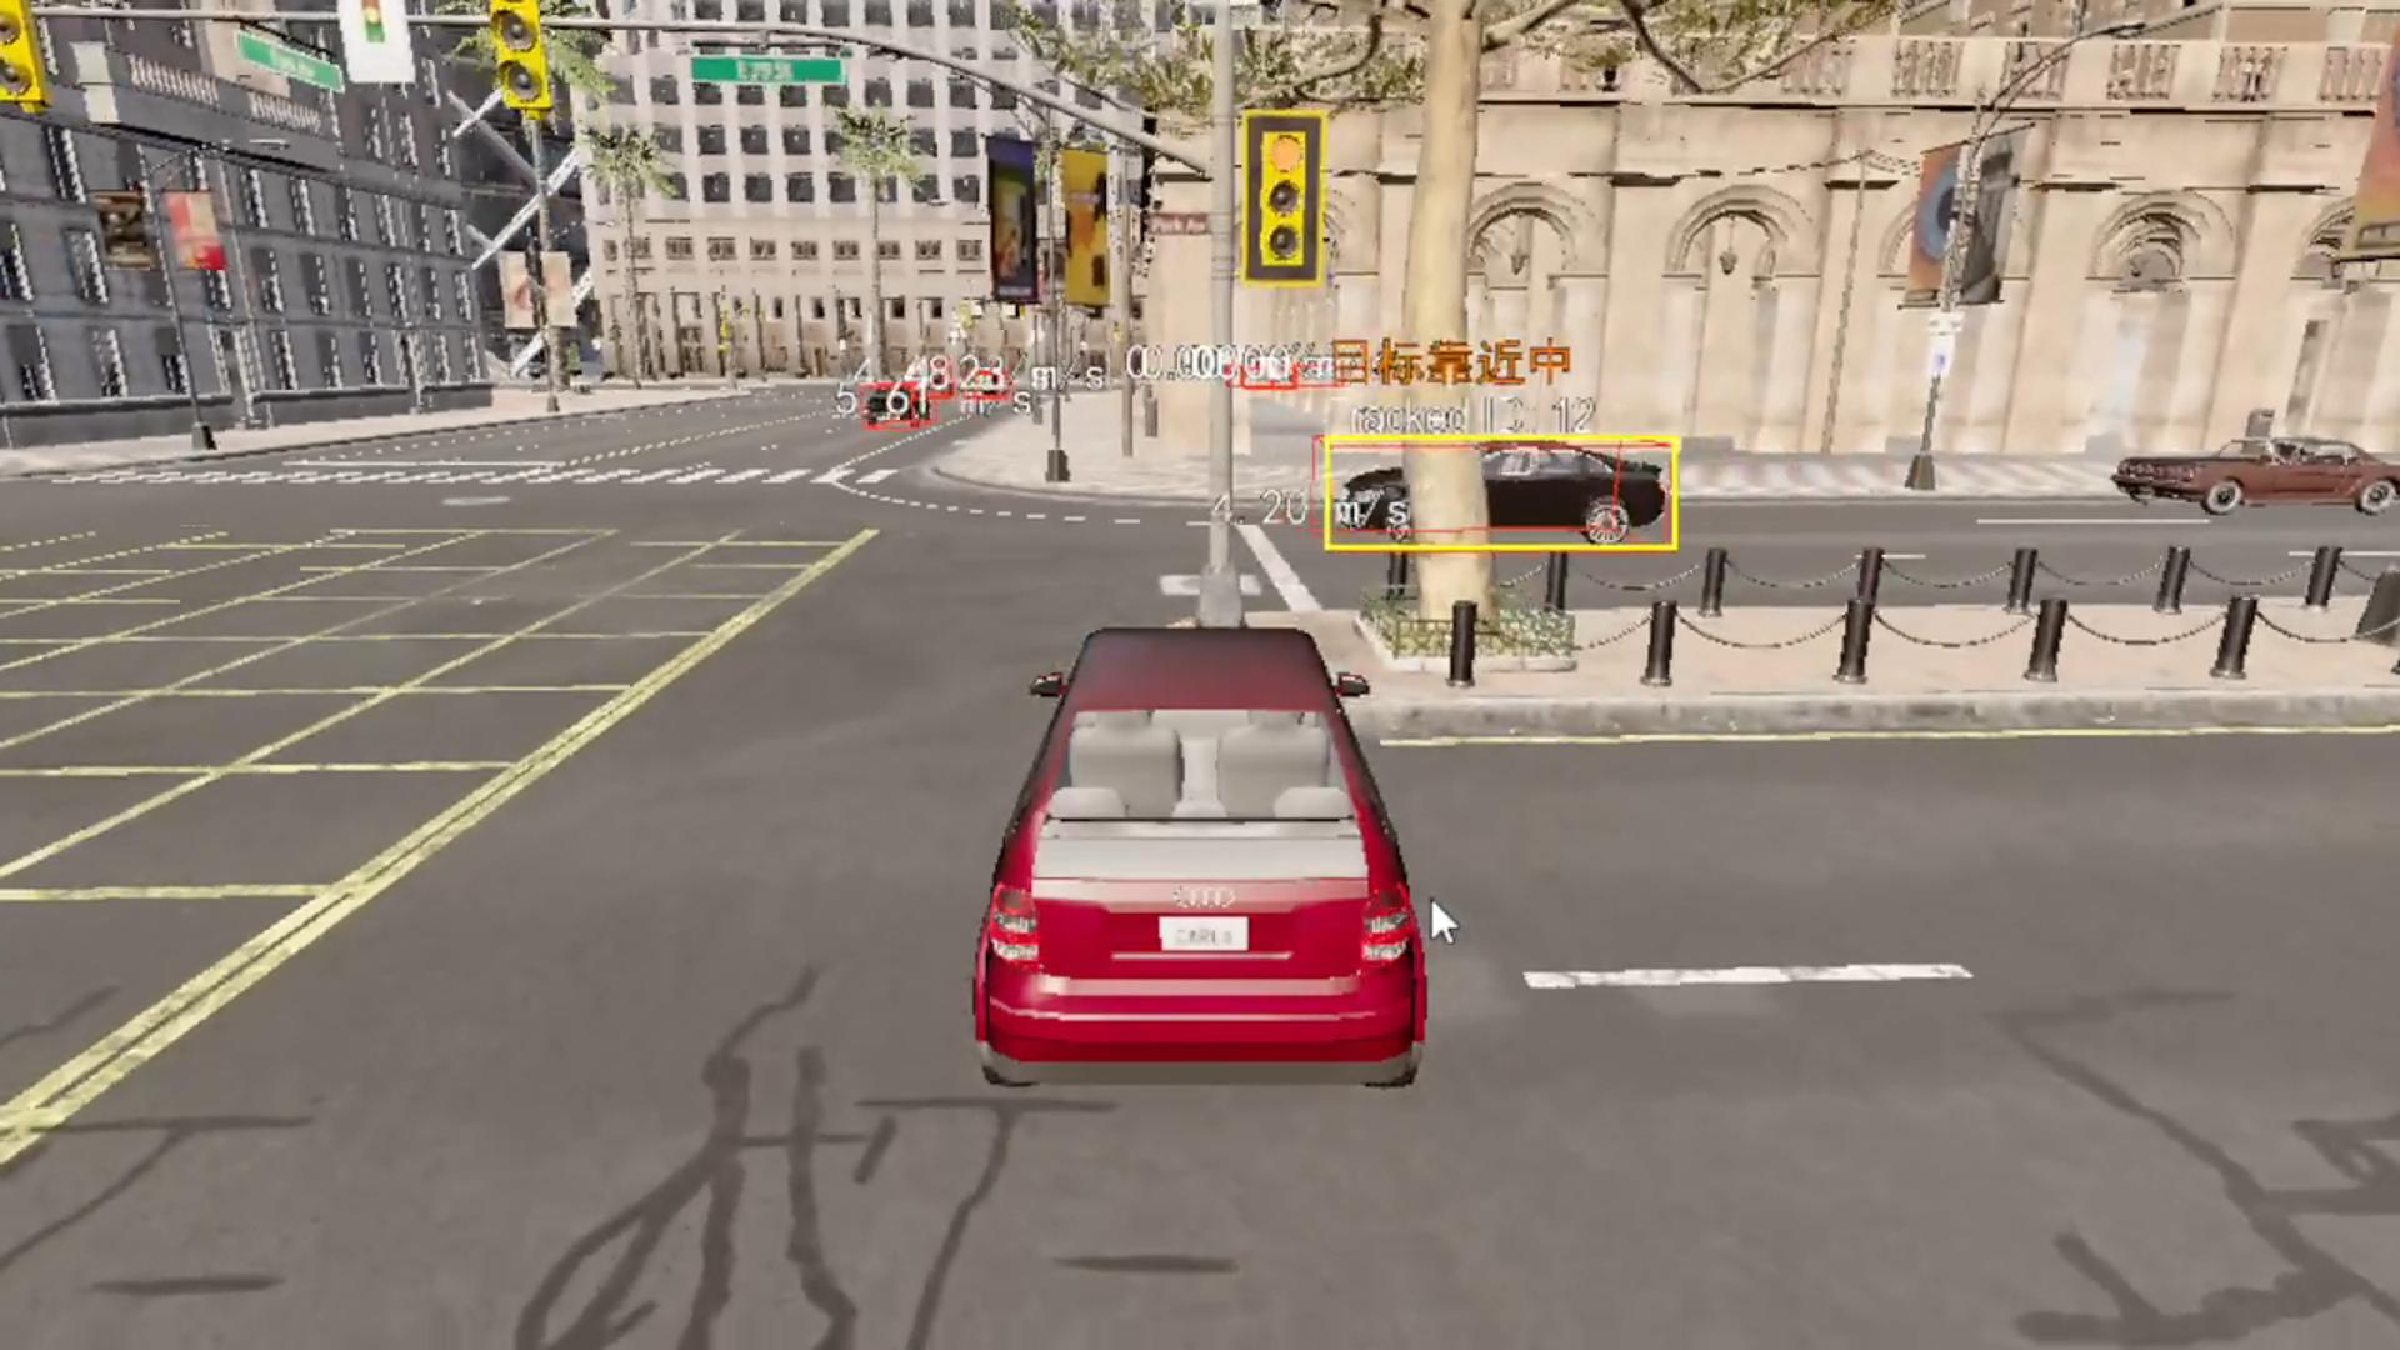
\includegraphics[width=1.0\textwidth]{images/遮挡已跟踪.pdf}  % 引用转换后的 PDF 文件
	\caption{遮挡下优化算法跟踪效果}
	\label{fig:covered2}  % 可用于引用此图片
\end{figure}

从整体实验结果来看,本文所提出的改进算法在目标 ID 管理的连续性方面优于传统 DeepSORT,尤其在遮挡、交错行驶等复杂场景中展现出更高的跟踪稳定性与准确性,为后续的交通行为分析与意图识别提供了更可靠的数据支持。


本文凭借跟踪评价标准展开比较,重点比较SORT算法、DeepSORT算法以及本文所提出的改进算法在若干跟踪指标上的差异,从表~\ref{tab:performance} 可看出,相较于原始的DeepSORT算法,本文的改进算法在IDF1上提升了2.8\%,在IDP上提升了3.2\%,在IDR上提升了2.6\%。跟踪过程中未出现ID切换情况,改进后的算法在跟踪精度上更具优势,从IDF1值并结合跟踪过程而言,SORT算法在跟踪车辆时,一旦车辆出现遮挡便无法继续跟踪,目标再次出现时只会被当作新目标进行跟踪,DeepSORT算法在跟踪车辆过程中,当车辆遮挡后重新出现的一段时间内会错误识别目标,随后才能正确跟踪。本文改进的算法在跟踪车辆过程中,从遮挡后到重新出现始终未出现错误识别,总的来说,DeepSORT算法与的改进算法都可有效跟踪出现遮挡情况下的车辆,不过在跟踪精度方面,本文提出的改进算法表现更为出色。
\begin{table}[H]
	\caption{跟踪算法性能对比表}
	\label{tab:performance}
	\centering
	\begin{tabular}{llllllll}
		\toprule
		  & IDF1\uparrow & IDP\uparrow & IDR\uparrow & IDSW\downarrow & MOTA\uparrow & FP\downarrow & FN\downarrow \\
		\midrule
		SORT & 81.7\% & 92.5\% & 73.1\% & 2 & 75.7\% & 87 & 1182\% \\
		DeepSORT & 83.7\% & 94.7\% & 74.9\% & 2 & 75.7\% & 88 & 1180\% \\
		Ours & 86.5\% & 97.9\% & 77.5\% & 0 & 75.8\% & 87 & 1178\% \\
		\bottomrule
	\end{tabular}
\end{table}

\subsection{跟踪效率分析}

在多目标跟踪的实际应用场景当中,一般都要求跟踪算法可实现实时跟踪,实时目标跟踪需要维持一定的帧率,一般,每秒 30 帧以上的帧率才可被视作实时跟踪,在追求多目标跟踪高精度的过程中,跟踪速度同样不容忽视,基于此,本文针对储备池的帧数展开量化分析,此前的内容曾提及,保存多帧目标特征虽可提升跟踪精度,然而复杂的计算量会致使跟踪速度迟缓,难以契合实时跟踪的需求。本文对目标特征帧数的参数选取进行测试,从表~\ref{tab:Ntest} 可看出,若仅保存一帧目标特征,极易出现偶然状况,比如保存的最后一帧特征是不完全的船体,这很容易导致匹配出错,当 N 取值为 10、20 乃至更大时,跟踪精度达到饱和状态,而跟踪速度却无法契合实时要求。当 N = 3 和 5 时,跟踪精度较高且能契合实时需求, N 为 5 是较为合适的选值,若要追求更快的跟踪速度,可将 N 设为 3。
\begin{table}[H]
	\caption{N值测试表}
	\label{tab:Ntest}
	\centering
	\begin{tabular}{lll}
		\toprule
		N(frame)  & IDF1(\%)  & FPS \\
		\midrule
		1 & 81.702 & 41 \\
		3 & 86.500 & 35 \\
		4 & 86.501 & 31 \\
		10 & 86.502 & 25 \\
		20 & 86.504 & 17 \\
		\bottomrule
	\end{tabular}
\end{table}

\section{跟踪与意图分析算法验证}

\subsection{验证准备}

本实验依靠Carla仿真平台及其Python接口开展,重点围绕视觉目标跟踪及行为意图识别展开融合工作,从而创建起一套具有即时性与可视化特征的自动驾驶感知子系统,此系统能够在Carla环境里达成目标感知,意图推断以及图形界面交互这样一种完整的循环过程,进而给后面的风险决策或者辅助控制供应先验方面的输入信息。

系统以 client\_bounding\_boxes.py作为主控脚本,它的运作流程包含如下一些重要步骤:

仿真环境初始化: 程序先通过 carla.Client 和 Carla 仿真服务创建起联系,再把预先指定好的地图场景(诸如 Town10)给加载进来,接着生成代表我方车辆(egovehicle)以及周围环境中的交通流,设置好摄像头之类的传感器之后开启同步模式。

实时图像获取与处理: 车辆前置RGB摄像头持续采集画面帧图,系统凭借Carla原生的投影功能从场景当中获取每辆车的3D边界框,并把它投影到图像平面上,以此当作检测输入。

目标选择与跟踪处理: 系统通过图像中心最近原则选定一个主目标当作跟踪对象,再用DeepSORT算法实施跨帧关联,守住稳定的目标ID。
行为意图识别: 依靠跟踪到的信息,再加上目标速度,运动方向以及中心点位移的改变情况,用物理建模的办法来做行为趋向判断,给出“靠近”“远离”“危险靠近”之类的表述。

可视化与数据记录: 系统把全部边界框,目标编号以及意图分析文字及时画到主界面上,用户可以用键盘来操控车辆行驶,而且系统每隔一定帧数就会把图像和标注信息自动存成数据集,以供后面训练和评价时使用。

图像渲染环节利用Pygame完成,该部分把图像帧,边界框,速度信息,追踪ID以及意图结果等相关元素加以整合,然后一并绘制到显示窗口上,从而生成出清晰易懂的运行界面,为了给后续的模型训练及效果回溯给予支撑,系统内部设置有自动保存图像帧和标注信息的功能,它会按照规定的间隔将图像以及包含边界框和速度信息的JSON格式文件存入本地数据集文件夹之中。而且,系统还加入了针对各个模块执行时间的统计功能,每当一帧处理结束之后就会输出各个阶段所花费的时间,当系统运行过一定数量的帧数之后,就会把所有时间段的详细信息整理成一张CSV表格并保存下来,方便使用者展开性能方面的分析与改良工作。

通过以上流程的达成,本系统既在仿真环境下做到了从感知到认识直至警报的全过程闭合,又有着较好的可视化表现能力和运行稳定程度,从而给后面章节里的功能演示以及性能评价形成牢靠根基。

\subsection{结果展示}

系统基于 pygame 实现实时渲染窗口,在 Windows 系统上运行稳定,图像帧率维持在约 30\textasciitilde40 FPS。在主界面中,用户可清晰看到如下信息:

\textbf{•前视图图像帧:}显示本车前方道路环境、其他车辆等元素;

\textbf{•目标边界框:}每个检测到的车辆被标注为 3D 投影框;

\textbf{•跟踪目标编号:}被追踪目标在框上方显示 Tracked ID;

\textbf{•意图分析结果:}在跟踪目标框的上方显示当前系统判断的意图(如“危险靠近”、“目标远离中”等);

\textbf{•速度信息显示:}在边界框上标记目标当前速度(单位:m/s);

\textbf{•系统状态输出:}在终端控制台实时输出当前帧耗时、目标状态等信息,辅助调试与评估。

用户能够用键盘来操控本车的行为(比如油门,刹车,转向等),以此考察系统处于各种驾驶状态时的感知鲁棒性,要想验证本系统在Carla仿真平台上的运行情况,本节通过一组功能界面截图表现系统的重要功能模块以及动态交互过程,在系统运行期间,各个模块相互协作去执行车辆环境感知,目标筛选,轨迹追踪和行为意图判断,从而创建起稳定的视觉处理及风险提示体系。

\begin{figure}[H]
	\centering
	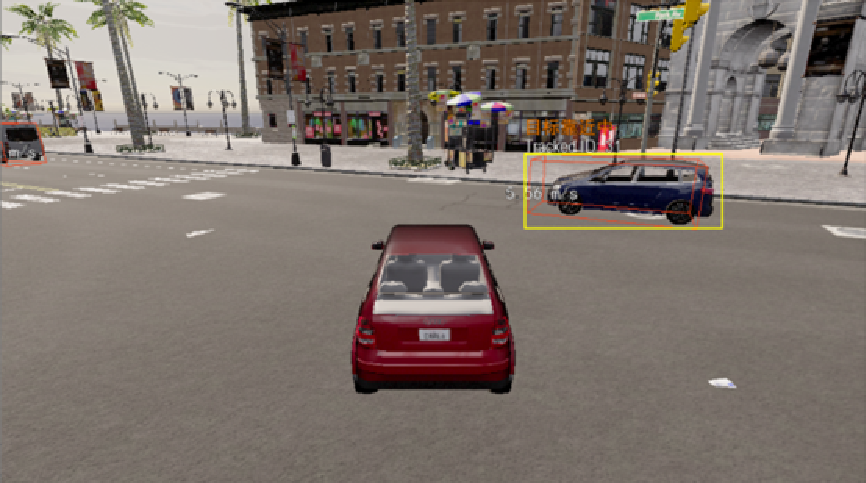
\includegraphics[width=0.8\textwidth]{images/图13 意图识别演示图(目标靠近).pdf}  % 引用转换后的 PDF 文件
	\caption{意图识别演示图(目标靠近)}
	\label{fig:example_image}  % 可用于引用此图片
\end{figure}

\begin{figure}[H]
	\centering
	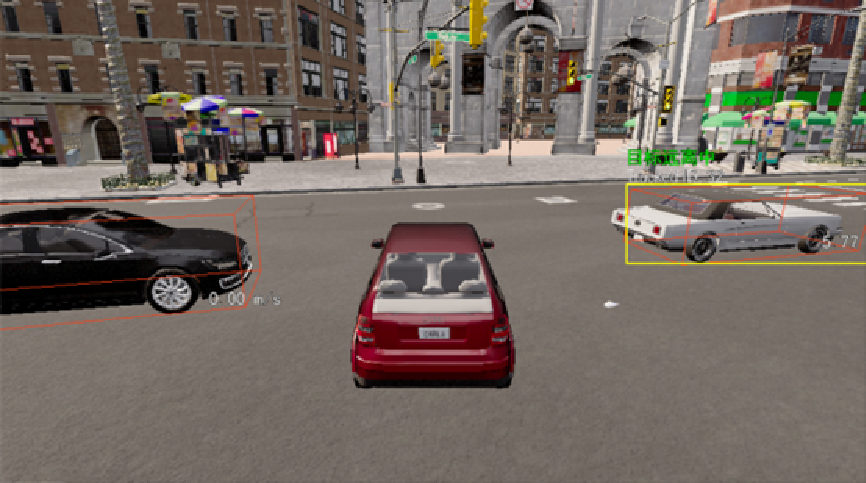
\includegraphics[width=0.8\textwidth]{images/图14 意图识别演示图(目标远离).pdf}  % 引用转换后的 PDF 文件
	\caption{意图识别演示图(目标远离)}
	\label{fig:example_image}  % 可用于引用此图片
\end{figure}

\begin{figure}[H]
	\centering
	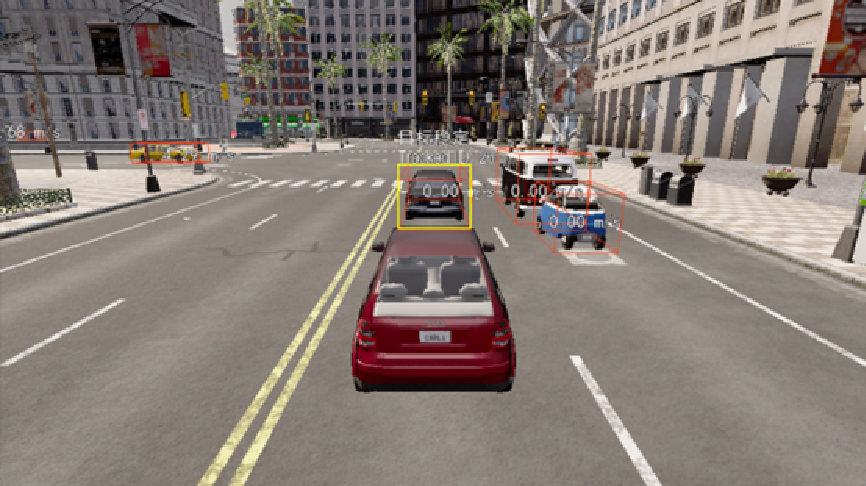
\includegraphics[width=0.8\textwidth]{images/图15 意图识别演示图(目标稳定).pdf}  % 引用转换后的 PDF 文件
	\caption{意图识别演示图(目标稳定)}
	\label{fig:example_image}  % 可用于引用此图片
\end{figure}

\section{整体算法性能评估}

为了系统性地评估本文所构建的视觉目标检测与跟踪模块的性能,实验从处理效率与运行稳定性两个维度展开。性能评估基于 Carla 仿真平台,在 Town10 和 Town01 等典型城市场景中进行,所有实验均在本地 Windows 平台(CPU:Intel i7-10750F,GPU:NVIDIA RTX 2060,内存 16GB)执行,未启用 GPU 加速推理,测试结果具备代表性。

\subsection{系统帧处理时序分析}

图~\ref{fig:frame} 展现了系统处理一帧图像数据时完整的流程及其各个阶段所耗费的时间,其中包含从仿真推进开始,通过图像获取,目标检测,目标跟踪,意图推断直到用户界面渲染结束这一整套过程,为精准度量性能,每个模块在主循环里设置了高精度计时器,用以记载时间戳,并算出相邻阶段之间所耗的时间,从而形成起帧处理的时序图。

\begin{figure}[H]
	\centering
	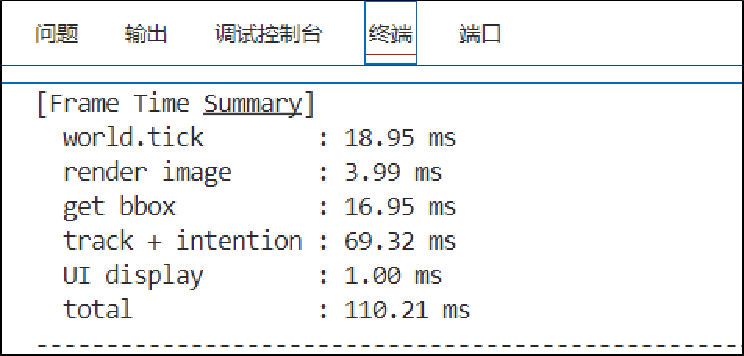
\includegraphics[width=0.8\textwidth]{images/图11 帧处理时序输出图.pdf}  % 引用转换后的 PDF 文件
	\caption{帧处理时序输出图}
	\label{fig:frame}  % 可用于引用此图片
\end{figure}

将时序输出图转化成对应统计表格分析可知,单帧总处理时间为 110.21 毫秒,系统整体运行帧率约为 9.09 FPS,接近准实时运行性能要求。其中,各子模块平均耗时如下:

\begin{table}[htbp]
	\caption{模块时序统计表}
	\label{tab:timetable}
	\centering
	\begin{tabular}{lll}
		\toprule
		模块名称 & 平均耗时 & 比例估算 \\
		\midrule
		场景同步(tick) & 18.95ms & 17.2\% \\
		图像渲染(render) & 3.99ms & 3.6\% \\
		边界框生成(bbox) & 16.95ms & 15.4\% \\
		跟踪与意图分析 & 69.32ms & 62.9\% \\
		界面刷新(UI) & 1.00ms & 0.9\% \\
		总计(Total) & 110.21ms & 100\% \\
		\bottomrule
	\end{tabular}
\end{table}

场景同步(tick):平均时耗达到了5.98ms,其用途在于同Carla仿真服务器保持同步,并推动仿真世界向前迈进一帧,这一部分属于系统的基础性操作范畴,时耗较为稳定,基本上不会受到仿真地图复杂程度以及传感器数量之类因素的左右。

图像渲染(render):平均时耗达3.99ms,其职能在于把图像传感器所传回来的原始BGRA数据加以剖析,转换成RGB形式,再转变成pygame能够渲染的格式,从而交给后面的处理环节去做后续工作,这个阶段的性能比较稳定,属于图像类任务的一种常见开销。

边界框生成(bbox):平均时耗达11.97ms,利用Carla自身具备的3DBoundingBox投影功能,从真实车辆模型创建顶点坐标,并把这些坐标投影到摄像机图像平面上,这种做法取代了依靠图像的传统目标检测网络,明显减小了计算量,还改良了标注的准确性,给后续的跟踪供应了稳定的输入。

跟踪与意图分析(track + intention):这个模块所耗费的时间很多,达到了90.33ms,大约占据总帧处理时间的80\%,其过程包含DeepSORT的轨迹维持和状态更新(卡尔曼滤波,Hungarian符合,轨迹结合),还有依靠目标运动状态的意图判断逻辑(距离变化率,速度阈值,靠近风险判断等等),这个阶段耗时太多是影响帧率的关键因素,必要着重加以改善。

用户界面刷新(UI):平均耗费时间只有1.00ms,其功能在于把文字信息以及边界框显示到屏幕之上,这部分开销十分微小。

\subsection{模块耗时对比分析}

要想进一步明晰各个模块在资源占用上的相对贡献度,于是把连续100帧的平均耗时统计结果制成了柱状图(~\ref{fig:time} ),从图上可以看出,DeepSORT跟踪模块以及意图推断阶段所占比例最大,这就表示,在以后的改良过程当中,应该最先考量针对这个模块展开算法提速或者模型压缩。

\begin{figure}[H]
	\centering
	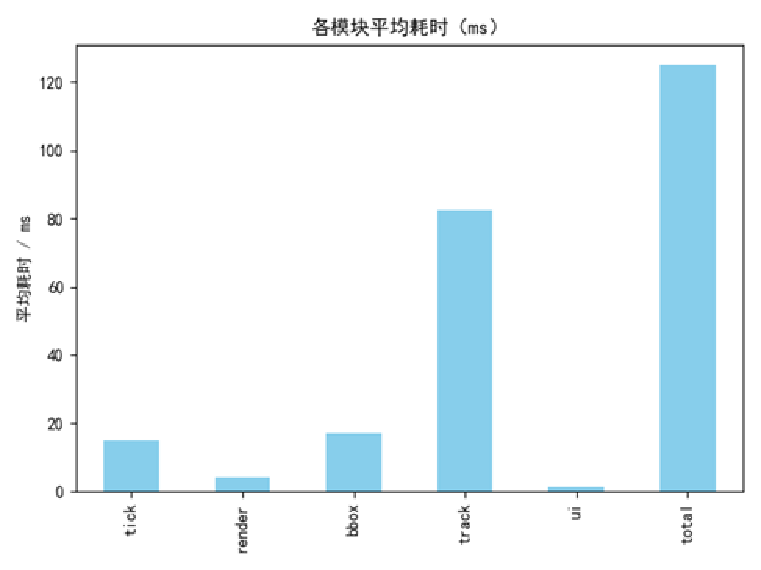
\includegraphics[width=0.8\textwidth]{images/图12 耗时统计柱状图.pdf}  % 引用转换后的 PDF 文件
	\caption{耗时统计柱状图}
	\label{fig:time}  % 可用于引用此图片
\end{figure}

可以看出,图像渲染、 边界框生成这类模块所耗费的时间比较少,这表明用Carla平台原本的三维boundingbox机制来取代图像检测模型是个有效的办法,既守住了高精度检测输入,又明显缩减了计算资源的占用量,界面渲染这个部分耗费的时间极少,可以在之后执行部署的时候关掉UI从而留出更多的处理能力。


\begin{tabular}{l l}
%  \verb|\songti| & {\songti 宋体} \\
%  \verb|\heiti| & {\heiti 黑体} \\
%   \verb|\kaiti| & {\kaiti 楷体}
\end{tabular}
